% =====================================================================
% revised_research_paper.tex  --  single self-contained source file
% Compile:  pdflatex revised_research_paper.tex  (run twice)
% Needs:    ./figures/  (all assets referenced below are in that folder)
% The bibliography is embedded (thebibliography), so no .bib file is needed.
% Items that the source material does not contain are marked with
% \todo{...} (red, bracketed). No such item has been filled with an invented value.
% =====================================================================
\documentclass[11pt,a4paper]{article}

\usepackage[T1]{fontenc}
\usepackage[utf8]{inputenc}
\usepackage{mathptmx}
\usepackage[margin=2.5cm]{geometry}
\usepackage{microtype}
\usepackage{amsmath,amssymb}
\usepackage{graphicx}
\usepackage{booktabs}
\usepackage{array}
\usepackage{xcolor}
\usepackage[font=small,labelfont=bf]{caption}
\usepackage{enumitem}
\usepackage{url}
\usepackage[colorlinks=true,linkcolor=blue!60!black,citecolor=blue!60!black,urlcolor=blue!60!black]{hyperref}

\setlength{\parskip}{3pt}
\setlist{itemsep=2pt,topsep=3pt}
\captionsetup[table]{position=top}
\captionsetup[figure]{position=bottom}
\renewcommand{\arraystretch}{1.08}
\graphicspath{{figures/}}

\newcommand{\todo}[1]{\textcolor{red}{[#1]}}
\newcommand{\IDF}{\mathrm{IDF1}}
\newcommand{\IDSW}{\mathrm{IDSW}}
\DeclareMathOperator{\cossim}{cos}

\title{\bfseries Evaluating Detector--Tracker Pipelines for Double-Count Suppression in Mango Orchard Video:\\
ByteTrack, Camera-Motion Compensation and a Prototype Re-Identification Memory}
\author{Derrick Samuel R. \qquad Prannavakhanth \qquad Priyanka Kaliraj\\[2pt]
Vellore Institute of Technology, Chennai}
\date{}

\begin{document}
\maketitle

% ---------------------------------------------------------------------
\begin{abstract}
Counting fruit from orchard video requires deciding, for every detection, whether it belongs to a fruit that has already been counted. Detector-only counting reports the same fruit in every frame in which it is visible, and short-term trackers fragment identities when foliage hides a fruit for many frames. We present OrchardVision, an implemented system for mango tracking in video. It couples a YOLO detector, interchangeable tracker back-ends (a centre-distance baseline, ByteTrack and TAPNext), optional camera-motion compensation (CMC), and an identity memory that keeps a prototype embedding per fruit so that a reappearing track can be linked back to a lost identity. Every intermediate result (detections, tracks, prototypes, re-identification events, per-frame timings, camera-motion estimates) is stored in SQLite and exposed through a REST API and an experiment harness, so that a counting error can be traced to the stage that caused it. We evaluate the tracker back-ends on three short orchard videos against a \emph{provisional} reference that was generated automatically by the same detector and has not been confirmed by a human annotator; the identity metrics therefore measure consistency with that reference, not absolute counting accuracy. With ByteTrack, the predicted track count exceeded the reference on all three videos (absolute errors of 1, 11 and 3 on reference counts of 9, 7 and 14; $+50\%$ when pooled). The centre-distance baseline scored marginally higher than ByteTrack (IDF1 70.9 vs.\ 69.0; HOTA 75.9 vs.\ 73.0) with fewer identity switches (1.0 vs.\ 5.7), a difference that three videos cannot resolve statistically. CMC changed mean IDF1 and HOTA by $+0.3$ and $+0.6$ points while raising mean identity switches from 5.7 to 17.3. The identity memory is implemented but is not part of the evaluated loop, and the TAPNext results and the re-identification threshold sweep are unverified and are not interpreted; cross-session matching is future work.
\end{abstract}

\noindent\textbf{Keywords:} fruit counting; multi-object tracking; re-identification; camera-motion compensation; precision agriculture; mango orchard.

% =====================================================================
\section{Introduction}\label{sec:intro}

\subsection{Research background}
Fruit count underpins yield forecasting, harvest logistics and crop-load management. In practice it is still commonly estimated by counting a small sample of trees by hand and extrapolating to the block. Fruit load varies strongly between trees and rows, so such sampling is slow and statistically weak. A camera carried by hand, on a vehicle or on an aerial platform samples an orchard far more densely, but turning footage into a count is not a matter of running a detector on every frame: one fruit stays in view for dozens or hundreds of consecutive frames and is reported each time. The central difficulty is therefore one of \emph{identity}: is a detection in the current frame a fruit that has been counted already, or a new one?

\subsection{Global impact}
The question has reach beyond a single orchard. The Food and Agriculture Organization (FAO) reports that an estimated 99 percent of tropical-fruit production originates in developing countries, predominantly in Asia and Latin America, and it tracks mango as one of four major tropical fruits together with avocado, papaya and pineapple~\cite{fao_tropical}. Where manual counting is labour-intensive, a count obtained from video could complement tree-level sampling. Video counting has already been demonstrated for mango: Wang et~al.\ combined a mango detector with a Kalman filter and the Hungarian algorithm and, on a 21-tree row, counted 2{,}050 fruit against a harvest tally of 3{,}286, roughly 62\% of the harvested fruit~\cite{wang2019mango}. The remaining gap between video counts and harvest counts is the practical motivation for studying where identity errors come from. We note that this paper does not measure yield accuracy; the contribution is a traceable pipeline and an honest evaluation of its tracking stage.

\subsection{Research gap}
Tracking-by-detection is the standard remedy for double-counting: a tracker links detections into trajectories and the count is the number of trajectories. Three properties of orchards make this fragile. Foliage hides fruit for tens of frames, which breaks trajectories and inflates the count on reappearance. Handheld and vehicle-mounted cameras move constantly, which disturbs motion models. Fruit on one tree look alike, which weakens appearance cues. Most tracking research was designed and evaluated on pedestrians and vehicles~\cite{bewley2016sort,wojke2017deepsort,zhang2022bytetrack,aharon2022botsort}. Among the works reviewed in Section~\ref{sec:related}, we found none that persists tracks, identity prototypes, re-identification events, per-frame timing and camera-motion estimates in a queryable form together with a harness that repeats a tracker comparison on the same video. That combination, and the diagnostic ability it gives, is the gap this work addresses; it is a systems-and-evaluation gap rather than a claim of a new tracking algorithm.

\subsection{Proposed approach}
OrchardVision processes a video in a single streaming pass. A YOLO detector~\cite{redmon2016yolo,ultralytics} proposes fruit; a tracker (selectable per job) links them; an optional step compensates global camera motion before tracking; and an identity memory represents each fruit by a unit-norm prototype embedding with quality statistics. A track that appears after another was lost may inherit the lost identity if appearance similarity and a motion gate both allow it, and tracks that overlap in time can never share an identity. All intermediate artefacts are persisted. The experiment harness then runs several trackers over the same video and scores them with IDF1, HOTA, identity switches and count error.

\subsection{Major contributions}
\begin{itemize}
\item \textbf{Traceable pipeline design.} A pipeline that couples detection, a pluggable tracker, optional camera-motion compensation and a prototype-based identity memory, in which detections, tracks, prototypes, per-sighting observations, re-identification events, per-frame timings and camera-motion estimates are stored as separate records (Section~\ref{sec:methods}). This allows a counting error to be traced to the stage that produced it.
\item \textbf{Repeatable tracker comparison.} An experiment harness and offline scripts that score tracker back-ends on identical video with IDF1, HOTA, identity switches and count error (Sections~\ref{sec:setup} and~\ref{sec:results}).
\item \textbf{A transparent evaluation on three mango videos.} Detector selection, a centre-distance / ByteTrack comparison, a CMC on/off ablation, a detection-threshold sweep, counting error and runtime, each reported against a reference whose construction is described and whose limits are stated (Sections~\ref{sec:setup}--\ref{sec:stats}).
\item \textbf{Negative and null findings, quantified.} On this reference, ByteTrack did not outperform a centre-distance baseline, CMC changed IDF1 and HOTA by under one point while tripling identity switches (5.7 to 17.3), and ByteTrack over-counted on every video (pooled $+50\%$). Section~\ref{sec:stats} shows why three videos cannot support significance claims in either direction.
\item \textbf{An explicit boundary of the claims.} The identity memory, the ReID-threshold sweep, TAPNext and cross-session matching are not validated, and the paper lists the experiments needed to validate them (Sections~\ref{sec:ablation}--\ref{sec:limits}).
\end{itemize}

\subsection{Paper organisation}
Section~\ref{sec:related} reviews related work. Section~\ref{sec:gap} separates existing techniques from the contributions of this paper. Section~\ref{sec:methods} describes each method in turn, with its architecture, formulation and configuration. Section~\ref{sec:setup} gives the data, hardware, reference construction and metrics. Section~\ref{sec:results} reports results method by method, and Section~\ref{sec:stats} analyses them statistically. Sections~\ref{sec:ablation} and~\ref{sec:hyp} cover the ablation and the hypotheses; Sections~\ref{sec:limits}--\ref{sec:conclusion} give limitations, impact, future work and conclusions. Appendix~\ref{app:unresolved} holds unresolved material and Appendix~\ref{app:discrepancies} lists source discrepancies.

% =====================================================================
\section{Related Work}\label{sec:related}

\paragraph{Fruit detection.} Deep detectors have replaced hand-crafted colour and shape features. Bargoti and Underwood applied Faster R-CNN to orchard imagery of mangoes, apples and almonds~\cite{bargoti2017deep}, and Koirala et~al.\ survey deep-learning methods for fruit detection and yield estimation~\cite{koirala2019review}. Single-stage detectors of the YOLO family~\cite{redmon2016yolo} are widely used for speed; we use the maintained Ultralytics implementation~\cite{ultralytics}. Per-frame detection carries no temporal identity.

\paragraph{Tracking-by-detection.} SORT associates detections across frames with a Kalman filter~\cite{kalman1960} for motion prediction and the Hungarian algorithm~\cite{kuhn1955} for assignment~\cite{bewley2016sort}; DeepSORT adds a learned appearance embedding to the association cost~\cite{wojke2017deepsort}. ByteTrack also associates low-confidence detections, which often correspond to partly occluded objects, to recover tracks that would otherwise be lost~\cite{zhang2022bytetrack}; this is relevant to fruit, where partial occlusion lowers detector confidence. BoT-SORT combines motion and appearance cues and adds camera-motion compensation, in which global image motion is estimated and used to correct motion predictions~\cite{aharon2022botsort}. These methods were designed and evaluated mainly for pedestrians.

\paragraph{Re-identification and point tracking.} Re-identification maps an image crop to an embedding in which crops of one identity are close; Hermans et~al.\ show that a carefully mined triplet loss is a strong baseline for person re-identification~\cite{hermans2017triplet}. An identity can be summarised by a prototype that aggregates its observations, and new detections can be compared with prototypes. Point-tracking methods follow a query point through occlusion; TAP-Vid is a benchmark for this task~\cite{doersch2022tapvid} and TAPNext formulates it as next-token prediction~\cite{zholus2025tapnext}. Tracking a point on a fruit surface could in principle be more stable under occlusion than tracking a bounding box; we treat TAPNext as one tracker option and do not interpret its results (Section~\ref{sec:results}).

\paragraph{Fruit counting from video.} Liu et~al.\ count fruit with a monocular camera by tracking fruit and associating them with a three-dimensional map to avoid double-counting~\cite{liu2019monocular}; this requires structure from motion, which can be brittle in foliage-rich scenes. Wang et~al.\ count mangoes in video with a detector, a Kalman filter and the Hungarian algorithm~\cite{wang2019mango}. OrchardVision takes an appearance- and motion-based route that needs no three-dimensional reconstruction and adds persistence of every intermediate result.

\paragraph{Metrics.} The CLEAR MOT metrics count identity switches (IDSW), false positives and misses~\cite{bernardin2008clear}. IDF1~\cite{ristani2016idf1} measures how long identities are correctly maintained (Eq.~\ref{eq:idf1}), and HOTA~\cite{luiten2021hota} balances detection and association quality (Eq.~\ref{eq:hota}). For counting, every identity switch changes the count, so IDF1 and IDSW are especially informative.

% =====================================================================
\section{Research Gap and Novelty}\label{sec:gap}

Table~\ref{tab:novelty} separates what is established, where it falls short for orchard fruit, how OrchardVision treats it, and what is new. We deliberately do not claim a new tracking algorithm or an accuracy improvement: the evidence in this paper does not support either.

\begin{table}[t]
\caption{Existing techniques, their limitations for orchard fruit, and the treatment in this paper.}\label{tab:novelty}
\centering\footnotesize
\begin{tabular}{p{2.6cm}p{3.8cm}p{4.2cm}p{3.6cm}}
\toprule
Established technique & Limitation for orchard video & Treatment in OrchardVision & Novelty status\\
\midrule
Kalman + Hungarian association~\cite{bewley2016sort} & Built for pedestrians; occlusion lasting tens of frames fragments tracks & Used as the centre-distance baseline and inside ByteTrack & Not novel\\
Low-score association (ByteTrack)~\cite{zhang2022bytetrack} & Evaluated mainly on pedestrians & Selectable back-end, evaluated on mango video & Not novel; evaluation on mango is new data\\
Camera-motion compensation~\cite{aharon2022botsort} & Effect on fruit identities not quantified here in prior work reviewed & Optional step with on/off ablation (Sec.~\ref{sec:ablation}) & Evaluation is new; mechanism is not\\
Appearance prototypes / ReID~\cite{wojke2017deepsort,hermans2017triplet} & Fruit on one tree are visually similar & Prototype EMA with quality gating, cosine threshold, motion gate, no-overlap rule & Combination is implemented; \textbf{benefit not yet validated}\\
3D-map data association~\cite{liu2019monocular} & Needs structure from motion & Appearance-and-motion route without 3D reconstruction & Alternative route; not compared head-to-head\\
\midrule
Persisted, queryable intermediate results & Not found in the works reviewed together with a repeatable tracker harness & Separate records for detections, tracks, prototypes, ReID events, timings, camera shift & \textbf{Principal contribution (systems)}\\
\bottomrule
\end{tabular}
\end{table}

The measurable contributions are those of Section~\ref{sec:intro}: a system whose stages can be inspected individually, and an evaluation whose limits are stated quantitatively. The accuracy findings are largely null or negative, and we report them as such.

% =====================================================================
\section{Proposed System and Methods}\label{sec:methods}

Figure~\ref{fig:pipeline} gives the architecture. Stages 1--4 form the loop scored by the offline evaluation scripts; stages 5--6 are implemented but are not part of that loop; stages 7--8 store and expose results. The backend is a FastAPI~\cite{fastapi} service with a SQLAlchemy~\cite{bayer2012sqlalchemy} 2.0 data layer, the web client is a React and TypeScript application, and long jobs run as a background task or through a Celery queue. Uploaded videos and cached JPEG frames are kept on the local file system through a storage service that confines resolved paths to the upload directory; object storage is not implemented. Each job stores the configuration it ran with, and the harness stores each run's tracker, scenario and metrics and exports them as JSON or CSV.

\begin{figure}[t]
\centering
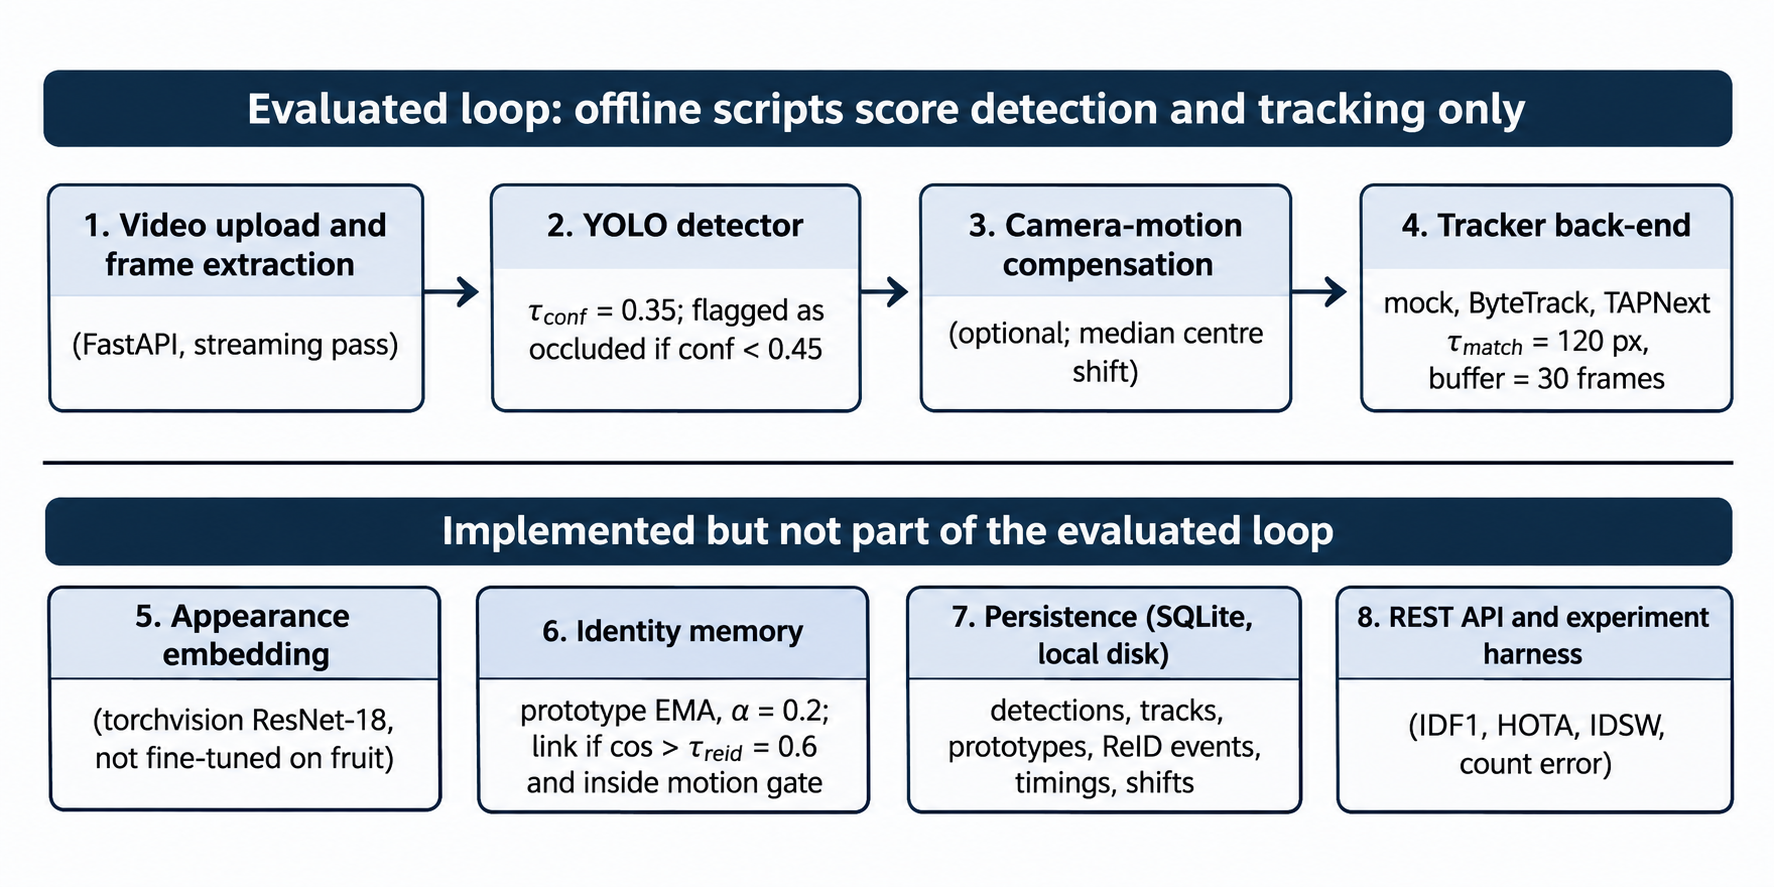
\includegraphics[width=\textwidth]{fig01_pipeline.png}
\caption{OrchardVision processing pipeline. Blue: stages scored by the offline evaluation. Orange (dashed): implemented stages that are not part of the evaluated loop. Parameter values are the defaults of Section~\ref{sec:methods}.}\label{fig:pipeline}
\end{figure}
\noindent Figure~\ref{fig:pipeline} makes the evidence boundary of this paper explicit: results in Section~\ref{sec:results} concern only the upper (blue) row. The embedder and identity memory below it affect no reported number. This diagram replaces the earlier version, whose boxes described operator steps (start services, upload, inspect, clean up) rather than data flow.

Each method below is described in the same order: overview, architecture and implementation, formulation, configuration, results (pointing to Section~\ref{sec:results}) and analysis. Methods are labelled as baseline, comparative or proposed.

\subsection{M1 -- YOLO detector (shared front end)}
\textbf{Overview.} All trackers receive the boxes of one detector, so tracker differences are not confounded with detector differences. \textbf{Architecture and implementation.} A YOLO model~\cite{redmon2016yolo,ultralytics} (Ultralytics implementation); the deployment default is YOLOv8n. A deterministic synthetic detector exists for development and tests and is not used for any real-video result. \textbf{Formulation.} For a detection with confidence $c$, the system keeps it if $c\ge\tau_{\mathrm{conf}}$ and flags it as occluded if $c<0.45$:
\begin{equation}
\mathrm{keep}(c)=\mathbb{1}[c\ge\tau_{\mathrm{conf}}],\qquad \mathrm{occluded}(c)=\mathbb{1}[c<0.45],\label{eq:conf}
\end{equation}
with $\tau_{\mathrm{conf}}=0.35$ by default. \textbf{Configuration and results.} Four training runs were logged (Section~\ref{sec:res-det}). \textbf{Analysis.} The occlusion flag is a confidence heuristic, not an occlusion measurement; it only feeds the observation-quality rule of M6.

\subsection{M2 -- Centre-distance association (baseline)}
\textbf{Overview.} A deterministic baseline (called ``mock'' in the code) that associates by centre distance; it is the simplest tracker in the study. \textbf{Architecture and implementation.} A detection is eligible to continue a track when its centre lies within $\tau_{\mathrm{match}}$ of the track's last centre, and an unmatched track is declared lost after $B$ frames:
\begin{equation}
\lVert \mathbf{c}_d-\mathbf{c}_k\rVert_2\le\tau_{\mathrm{match}},\qquad \tau_{\mathrm{match}}=120\ \text{px},\quad B=30 .\label{eq:gate}
\end{equation}
The source does not state how ties among eligible detections are resolved (e.g.\ greedy or optimal assignment). \todo{Assignment rule not stated in source.} \textbf{Experimental configuration.} Same videos, detector and threshold as the other trackers. \textbf{Results and analysis.} Section~\ref{sec:res-trk}: this baseline scored at least as high as ByteTrack on the averaged metrics.

\subsection{M3 -- ByteTrack (comparative)}
\textbf{Overview.} A tracking-by-detection method that also associates low-confidence detections with existing tracks~\cite{zhang2022bytetrack}. \textbf{Architecture and implementation.} Two-stage association built on a Kalman motion model and Hungarian assignment~\cite{kalman1960,kuhn1955}; the tracker back-end shares the interface and the parameters $\tau_{\mathrm{match}}$ and $B$ of Eq.~(\ref{eq:gate}) with the baseline. \textbf{Formulation.} We do not restate ByteTrack's equations; see~\cite{zhang2022bytetrack}. \textbf{Configuration.} ByteTrack's own high-confidence threshold is internal to the tracker; the source attributes the insensitivity of identity metrics to the detection threshold to it (Section~\ref{sec:res-thr}). \textbf{Results and analysis.} Sections~\ref{sec:res-trk}, \ref{sec:res-count}, \ref{sec:res-thr} and \ref{sec:res-time}.

\subsection{M4 -- TAPNext point tracking (comparative, unverified)}
\textbf{Overview.} TAPNext tracks point queries through the video as next-token prediction~\cite{zholus2025tapnext}; the system seeds queries from detections. \textbf{Architecture, formulation.} See~\cite{zholus2025tapnext}; no equations are restated. \textbf{Results.} The reported metrics are on a scale that could not be reconciled with the other rows (Table~\ref{tab:trackers}), so they are neither compared nor interpreted. \textbf{Analysis.} None is drawn; Section~\ref{sec:future} lists the re-run needed.

\subsection{M5 -- Camera-motion compensation (optional; ablation component)}
\textbf{Overview.} Removes global image motion before tracking so that camera movement is not seen as object motion. \textbf{Implementation.} Per frame $t$, the shift $\mathbf{s}_t$ is the median displacement of that frame's detection centres. Boxes are translated into a stabilised coordinate system before the tracker update and mapped back before storage:
\begin{equation}
\mathbf{s}_t=\operatorname{median}_i\bigl(\mathbf{c}^{t}_i-\mathbf{c}^{t-1}_i\bigr),\qquad \tilde{b}_t=b_t-\mathbf{S}_t .\label{eq:cmc}
\end{equation}
Here $\mathbf{S}_t$ denotes the accumulated shift up to frame $t$; the accumulation convention, and how centres are paired across frames, are not specified in the source. \todo{Pairing and accumulation details not stated.} \textbf{Configuration.} Switched on or off per job; on the three videos the median global shift is reported as 0.3~px on V1 and 4.5~px on V2 (95th percentile 44.7~px on V2). \textbf{Results and analysis.} Section~\ref{sec:res-cmc}.

\subsection{M6 -- Prototype identity memory (proposed; not evaluated)}
\textbf{Overview.} Gives each fruit a persistent identity so that a track appearing after another was lost can be re-associated with it.

\textbf{Architecture and formulation.} For each tracked detection an appearance embedding $\mathbf{e}_t$ is computed. Identity $k$ keeps a unit-norm prototype $\mathbf{p}_k$ updated as an exponential moving average with memory rate $\alpha$ (default 0.2):
\begin{equation}
\mathbf{p}_k\leftarrow\frac{(1-\alpha)\,\mathbf{p}_k+\alpha\,\mathbf{e}_t}{\lVert(1-\alpha)\,\mathbf{p}_k+\alpha\,\mathbf{e}_t\rVert_2}.\label{eq:proto}
\end{equation}
The quality of an observation is the detector confidence, multiplied by 0.55 when the detection is flagged as occluded; observations with quality below 0.3 are discarded before they can influence a prototype:
\begin{equation}
q_t=c_t\cdot\bigl(0.55\ \text{if occluded, else }1\bigr),\qquad \text{accept iff }q_t\ge0.3 .\label{eq:quality}
\end{equation}
An identity's quality is an exponential moving average of its accepted observations' qualities (the smoothing rate is not reported \todo{rate not stated}); the identity is marked \emph{confident} once it has at least three observations and quality of at least 0.5.

\textbf{Linking rule.} A new track receives the lowest unused identity number unless it is a plausible reappearance of a track reported lost, in which case it inherits that identity. Candidates are ranked by cosine similarity, which must exceed $\tau_{\mathrm{reid}}$ (default 0.6), and are then filtered by a motion gate whose radius grows with the occlusion length $\Delta$ (default parameters reported as 120~px and 45~px per frame, which we read as $r(\Delta)=120+45\,\Delta$ px; the functional form is our reading):
\begin{equation}
\text{link}\iff\cos(\mathbf{p}_k,\mathbf{e})>\tau_{\mathrm{reid}}\ \wedge\ \lVert\mathbf{c}_{\text{new}}-\mathbf{c}_{\text{lost}}\rVert_2\le r(\Delta)\ \wedge\ \text{no temporal overlap with identity }k .\label{eq:link}
\end{equation}
Accepted and rejected links are stored as re-identification events with their similarity. Tracks that overlap in time can never share an identity, which prevents two simultaneously visible fruit from being merged.

\textbf{Error modes.} A missed reappearance creates a new identity and over-counts; a false link across a long gap merges two fruit and under-counts. $\tau_{\mathrm{reid}}$ trades these errors against each other (Figure~\ref{fig:hyp}).

\textbf{Configuration and results.} The offline harness scores detection and tracking only, so no result for this method exists in this paper. The identity memory therefore has a \emph{data limitation}, not a negative result. Appendix~\ref{app:unresolved} reproduces an unverified table for transparency.

\subsection{M7 -- Appearance embedder}
In real mode the embedding is either a checkpoint at a configured path (producible with the repository's \texttt{train\_identity\_embedder.py} script) or, when none is present, a torchvision ResNet-18 feature extractor. The default configuration was used: a ResNet-18 that has \emph{not} been trained on fruit crops. An earlier project report also described contrastive (InfoNCE~\cite{oord2018cpc}) training with pseudo-labels from density-based clustering~\cite{ester1996dbscan}, whereas the evaluation described the untrained extractor and the conclusion listed fine-tuning as future work; we therefore claim no result from a trained embedder. Identity prototypes can be inspected in two dimensions by t-SNE~\cite{vandermaaten2008tsne} or, for few identities, a principal-component projection~\cite{jolliffe2016pca}. \todo{Source of the ResNet-18 weights (e.g.\ ImageNet) to be confirmed by the authors.}

\subsection{M8 -- Evaluation metrics}
Let IDTP, IDFP and IDFN be the true positives, false positives and false negatives of a global one-to-one matching between ground-truth and predicted trajectories:
\begin{equation}
\IDF=\frac{2\,\mathrm{IDTP}}{2\,\mathrm{IDTP}+\mathrm{IDFP}+\mathrm{IDFN}} .\label{eq:idf1}
\end{equation}
HOTA at localisation threshold $\beta$ is the geometric mean of detection accuracy and association accuracy, usually averaged over $\beta$:
\begin{equation}
\mathrm{HOTA}_\beta=\sqrt{\mathrm{DetA}_\beta\cdot\mathrm{AssA}_\beta} .\label{eq:hota}
\end{equation}
For video $v$ with $N_v$ provisional-reference identities and $\hat N_v$ predicted tracks, the count error used in Section~\ref{sec:res-count} is
\begin{equation}
E_v=\lvert\hat N_v-N_v\rvert,\qquad E^{\%}_v=100\,E_v/N_v .\label{eq:counterr}
\end{equation}
The module also implements identity switches, track fragmentation and identity recovery rate; only IDF1, HOTA, IDSW and count error are reported here.

% =====================================================================
\section{Experimental Setup}\label{sec:setup}

\subsection{Data}
Table~\ref{tab:videos} lists the three orchard videos. The table was flagged ``to be filled in'' in the source despite containing values, so it is provisional.

\begin{table}[t]
\caption{Evaluation videos. ``GT identities'' are machine-generated (Section~\ref{sec:gt}).}\label{tab:videos}
\centering\small
\begin{tabular}{lllrrrr}
\toprule
Video & Source file & Camera label$^{*}$ & Resolution & FPS & Frames & GT identities\\
\midrule
V1 & test & static & $960\times506$ & 29.9 & 747 & 9\\
V2 & test4 & static & $1366\times768$ & 24 & 141 & 7\\
V3 & Test3 & static & $768\times432$ & 24 & 337 & 14\\
\bottomrule
\end{tabular}\\[2pt]
{\footnotesize $^{*}$As printed in the source; the source also reports non-trivial global camera motion on these videos (Section~\ref{sec:res-cmc}).}
\end{table}

\begin{figure}[t]
\centering
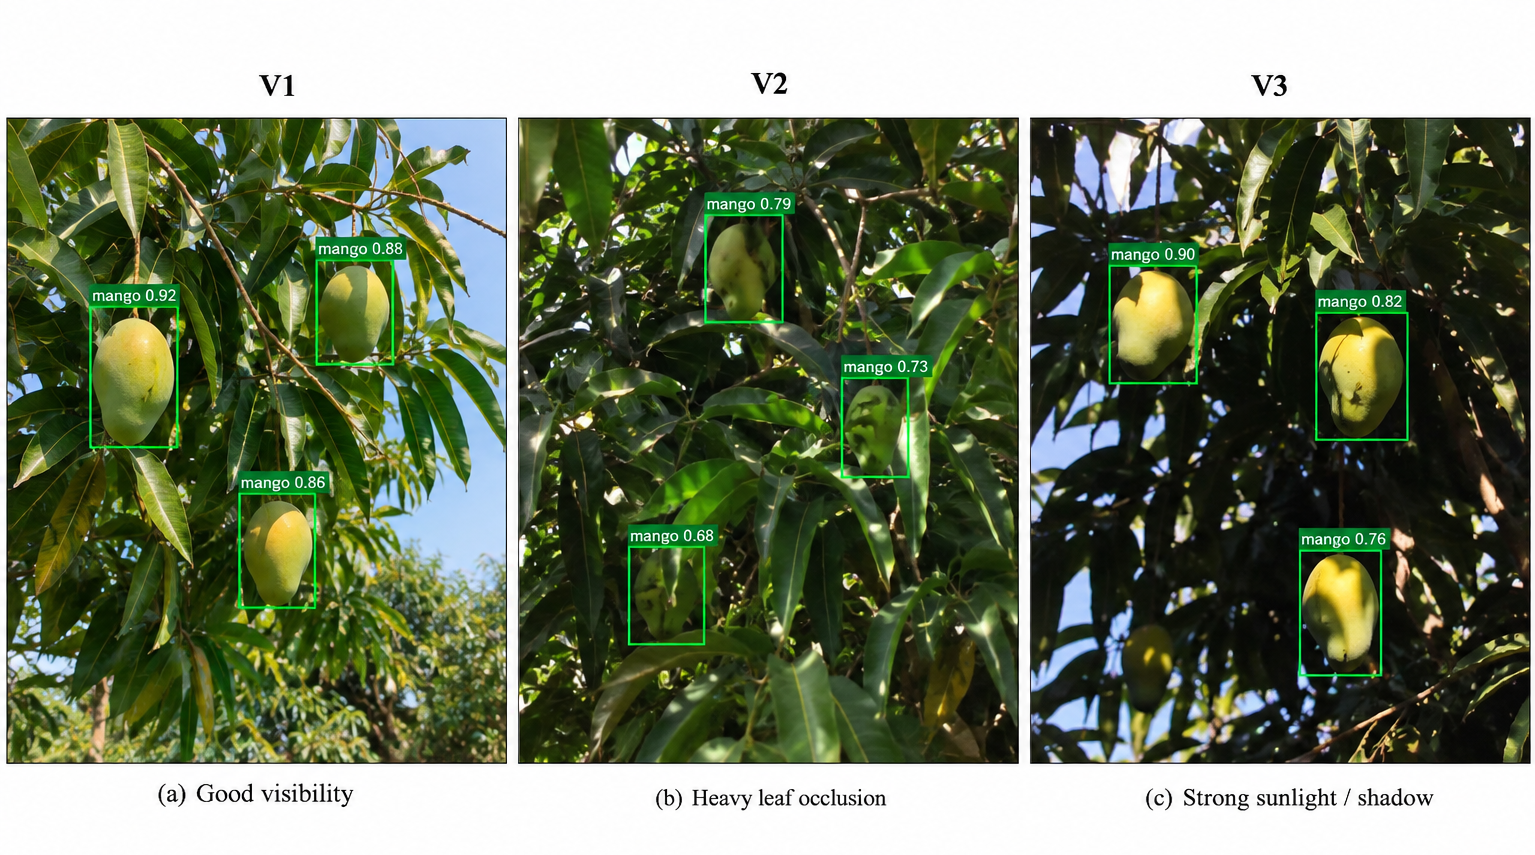
\includegraphics[width=.8\textwidth]{fig03_sample_frames.png}
\caption{Sample frames with detector output: (a) V1, good visibility; (b) V2, heavy leaf occlusion; (c) V3, strong sunlight and shadow.}\label{fig:frames}
\end{figure}
\noindent Figure~\ref{fig:frames} shows the three recording conditions. The detections carry confidences of roughly 0.7--0.9 on the displayed frames, with the lowest values on the heavily occluded V2 frame, in line with the use of confidence as an occlusion cue in Eq.~(\ref{eq:conf}).

\subsection{Hardware and software}
Tracking and runtime measurements were taken on one machine: Apple M2 Max (12-core CPU, 30-core GPU), 64~GB unified memory, macOS (Darwin 24, arm64), Python 3.12, PyTorch 2.14, Ultralytics 8.4. The detector training runs of Table~\ref{tab:detector} were executed on a separate Windows workstation whose specification was not logged.

\subsection{Provisional ground truth}\label{sec:gt}
The reference is machine-generated and has \emph{not} been confirmed by a human annotator. It was built by running the same YOLO detector over every frame, associating boxes at the full frame rate, and keeping identities that last at least fifty frames. The minimum-length rule removes the short tracks that occlusion and false positives create: on V1, raw association yielded 61 identities, of which 44 lasted fewer than twenty frames and nine lasted fifty frames or more. Table~\ref{tab:gt} summarises the construction.

\begin{table}[t]
\caption{Construction of the provisional ground truth: raw association output and identities kept by the minimum-length rule.}\label{tab:gt}
\centering\small
\begin{tabular}{lrrrrr}
\toprule
Video & Raw ids & Kept & Dropped & Boxes & Max concurrent\\
\midrule
V1 & 61 & 9 & 52 & 2956 & 10\\
V2 & 44 & 7 & 37 & 854 & 10\\
V3 & 43 & 14 & 29 & 1947 & 12\\
\bottomrule
\end{tabular}
\end{table}

Two consequences follow. First, because the reference comes from the same detector the system runs, identity metrics measure how consistently a tracker maintains identities that the detector proposes; they say nothing about whether the detector is right and are not absolute counting accuracy. Second, the reference is unreviewed: frames were exported every tenth frame for manual review, but that review has not been reported. Note also that the maximum number of concurrently visible reference objects (10, 10, 12) exceeds the kept identity count on V1 and V2, which is a further sign that the reference removes objects (Table~\ref{tab:gt}).

\subsection{Metrics}
For each tracker we report IDF1, HOTA and identity switches, averaged over V1--V3 (Eqs.~\ref{eq:idf1}, \ref{eq:hota}). For counting we compare the number of predicted tracks with the number of reference identities (Eq.~\ref{eq:counterr}).

% =====================================================================
\section{Results and Discussion}\label{sec:results}

\subsection{M1: detector training runs}\label{sec:res-det}
Four detector training runs were logged by Ultralytics (Table~\ref{tab:detector}): YOLOv8n (50 epochs), two YOLOv8m runs (10 and 93 epochs) and YOLOv8x (40 epochs). The YOLOv8n run reached the highest validation mAP$_{50\text{-}95}$ (0.827) and the lowest latency (33.6~ms) and is the default detector of the deployment. The runs are not a controlled comparison: the YOLOv8n and YOLOv8m runs were trained on a second, larger annotation set with different schedules, and the YOLOv8x run was logged only at its final epoch. The table justifies the deployment default but does not rank the architectures; the mAP$_{50\text{-}95}$ differences (0.788--0.827) are small and confounded with dataset and schedule.

\begin{table}[t]
\caption{Detector training runs. P, R and mAP are validation metrics at the best epoch; ``Best ep.'' is the best epoch within the run's total epochs. Latency is the median of ten forward passes of the exported weights at 640 pixels.}\label{tab:detector}
\centering\small
\begin{tabular}{lrrrrrrr}
\toprule
Run & Epochs & Best ep. & P & R & mAP$_{50}$ & mAP$_{50\text{-}95}$ & ms/frame\\
\midrule
mango\_yolov8n-4 & 50 & 49 & 0.946 & 0.975 & 0.985 & 0.827 & 33.6\\
mango\_yolov8m\_exp-2 & 10 & 10 & 0.928 & 0.949 & 0.979 & 0.808 & 83.5\\
mango\_yolov8m\_exp-3 & 93 & 73 & 0.958 & 0.971 & 0.987 & 0.789 & 83.5\\
mango\_yolov8x & 40 & 40 & 0.958 & 0.961 & 0.985 & 0.788 & 173.1\\
\bottomrule
\end{tabular}
\end{table}

\begin{figure}[t]
\centering
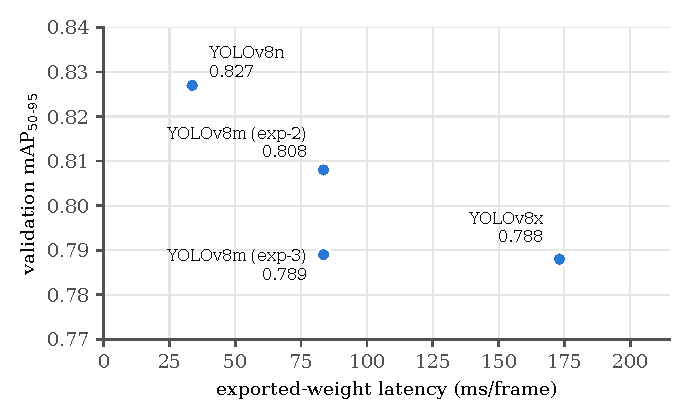
\includegraphics[width=.62\textwidth]{fig04_detector_tradeoff.pdf}
\caption{Validation mAP$_{50\text{-}95}$ against exported-weight latency for the four runs of Table~\ref{tab:detector}. Runs differ in dataset and schedule, so the plot is descriptive, not a controlled comparison.}\label{fig:detector}
\end{figure}
\noindent Figure~\ref{fig:detector} shows that YOLOv8n sits at the favourable corner (highest mAP$_{50\text{-}95}$, lowest latency), whereas latency grows roughly five-fold to YOLOv8x without a higher validation score. Because of the confounds above, this supports the choice of a small detector for a video pipeline, not a statement about model capacity.

\begin{figure}[t]
\centering
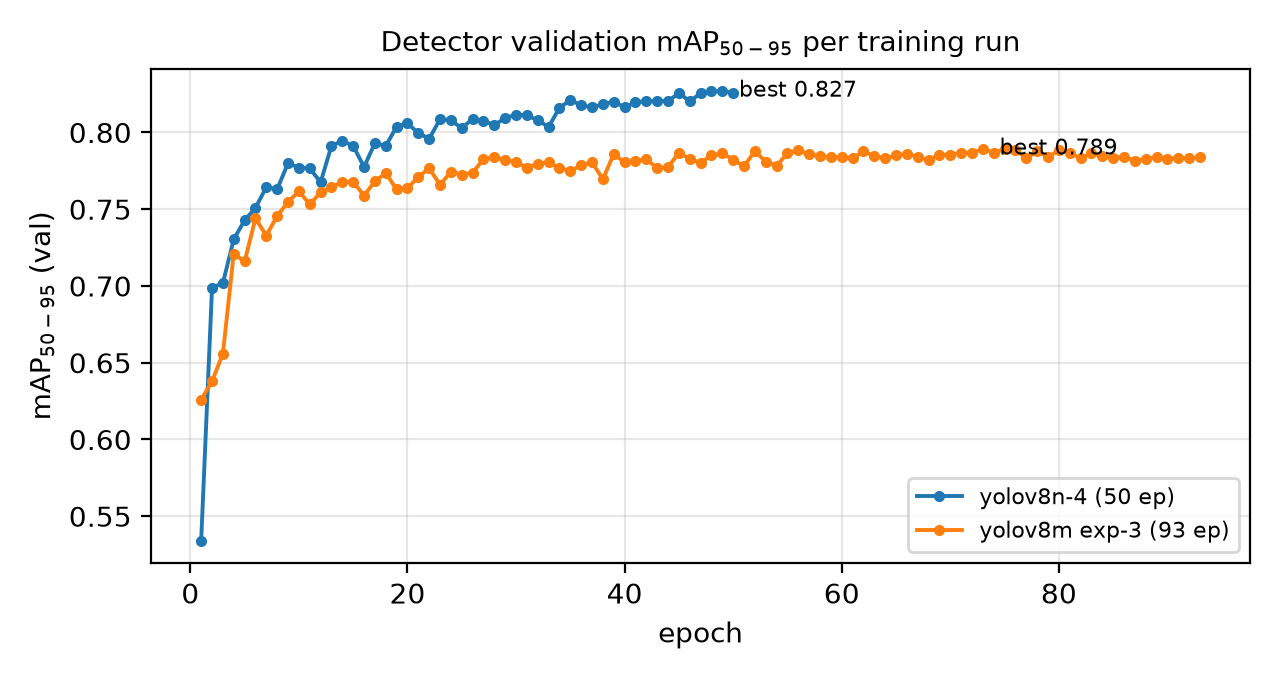
\includegraphics[width=.8\textwidth]{fig05_detector_curves.png}
\caption{Validation mAP$_{50\text{-}95}$ per epoch for the two longest detector runs (original training log plot).}\label{fig:curves}
\end{figure}
\noindent Figure~\ref{fig:curves} shows that both runs rise steeply in the first ten or so epochs and then change slowly; the YOLOv8n run (best 0.827) keeps improving slightly until its final epochs, while the YOLOv8m run (best 0.789 at epoch 73) is nearly flat after epoch 30.

\subsection{M2 and M3 (and M4): tracker comparison}\label{sec:res-trk}
Table~\ref{tab:trackers} compares the three tracker back-ends against the provisional ground truth, and Figure~\ref{fig:stats} gives the per-video values behind the averages for ByteTrack.

\begin{table}[t]
\caption{Tracker comparison, averaged over V1--V3, against the provisional full-rate ground truth. Count error is the source's mean absolute difference between predicted tracks and reference identities; its unit is unresolved (see Appendix~\ref{app:discrepancies}).}\label{tab:trackers}
\centering\small
\begin{tabular}{lrrrr}
\toprule
Tracker (role) & IDF1 & HOTA & ID switches & Count error\\
\midrule
centre-distance (baseline) & 70.9 & 75.9 & 1.0 & 0.67\\
ByteTrack (comparative) & 69.0 & 73.0 & 5.7 & 0.61\\
TAPNext (comparative)$^{\ddagger}$ & 0.88 & 0.89 & 3.2 & 0.55\\
\bottomrule
\end{tabular}\\[2pt]
{\footnotesize $^{\ddagger}$Unverified. The source column headings say ``(\%)'', but the TAPNext IDF1 and HOTA are printed as 0.88 and 0.89 while the other rows use a 0--100 scale. Whether TAPNext is on a 0--1 scale, is a percentage, or is a different quantity is unconfirmed, so the row is neither converted nor compared with the others.}
\end{table}

On ByteTrack, the per-video values reproduce the table averages exactly: IDF1 96.97, 22.56 and 87.43; HOTA 96.93, 33.25 and 88.87; and 2, 6 and 9 identity switches on V1, V2 and V3 (means 68.99, 73.02 and 5.67). For the centre-distance baseline only the average and the per-video switch counts (1, 0 and 2) are available in the source.

\begin{figure}[t]
\centering
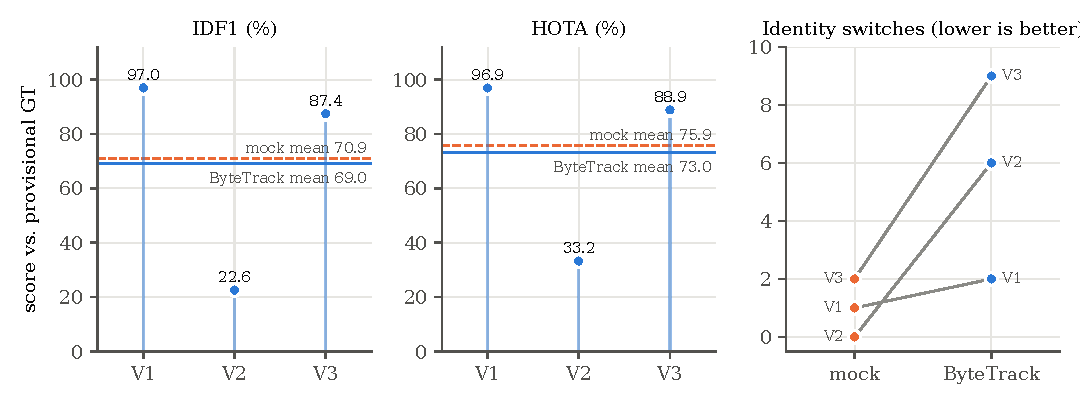
\includegraphics[width=\textwidth]{fig06_tracker_pervideo_stats.pdf}
\caption{Per-video tracker scores against the provisional reference. Left and centre: ByteTrack IDF1 and HOTA per video (dots), ByteTrack mean (solid line) and centre-distance mean from Table~\ref{tab:trackers} (dashed line; per-video baseline values are not available). Right: identity switches per video for both trackers, paired by video.}\label{fig:stats}
\end{figure}
\noindent Figure~\ref{fig:stats} shows that the averages hide a very uneven distribution. ByteTrack scores above 87 on V1 and V3 but only 22.6 (IDF1) and 33.3 (HOTA) on V2, the shortest and most occluded clip, and its identity switches rise from 2 to 9 across V1--V3. The baseline records fewer switches than ByteTrack on every video (1, 0, 2 against 2, 6, 9). The near-equality of the two averages therefore says little about any single scene; Section~\ref{sec:stats} quantifies how little three videos can say.

\paragraph{Analysis.} On this reference, the centre-distance baseline scored slightly higher (IDF1 70.9 vs.\ 69.0, HOTA 75.9 vs.\ 73.0) with fewer identity switches (1.0 vs.\ 5.7). The gaps are a few points from three videos, with no variance estimate and with a reference built by the same detector, so we do not conclude that either tracker is better; the data show no benefit of ByteTrack over simple association here. The TAPNext row supports no conclusion.

\subsection{M5: camera-motion compensation}\label{sec:res-cmc}
Table~\ref{tab:cmc} and Figure~\ref{fig:cmc} report the aggregate effect of compensation, averaged over V1--V3. With compensation, mean IDF1 changed from 68.9 to 69.2 and mean HOTA from 73.0 to 73.6, while mean identity switches rose from 5.7 to 17.3.

\begin{table}[t]
\caption{Effect of compensating camera motion, averaged over V1--V3. The shift of each frame is the median displacement of its detection centres; boxes are moved into stabilised coordinates before tracking and back before storage.}\label{tab:cmc}
\centering\small
\begin{tabular}{lrrr}
\toprule
Camera-motion mode & IDF1 (\%) & HOTA (\%) & ID switches\\
\midrule
Off & 68.9$^{\dagger}$ & 73.0 & 5.7\\
On (compensation applied) & 69.2 & 73.6 & 17.3\\
Difference (on $-$ off) & $+0.3$ & $+0.6$ & $+11.6$\\
\bottomrule
\end{tabular}\\[2pt]
{\footnotesize $^{\dagger}$Table~\ref{tab:trackers} gives 69.0 for the same configuration; the per-video values average to 68.987, so 68.9 is a truncation and 69.0 a rounding of the same number.}
\end{table}

\begin{figure}[t]
\centering
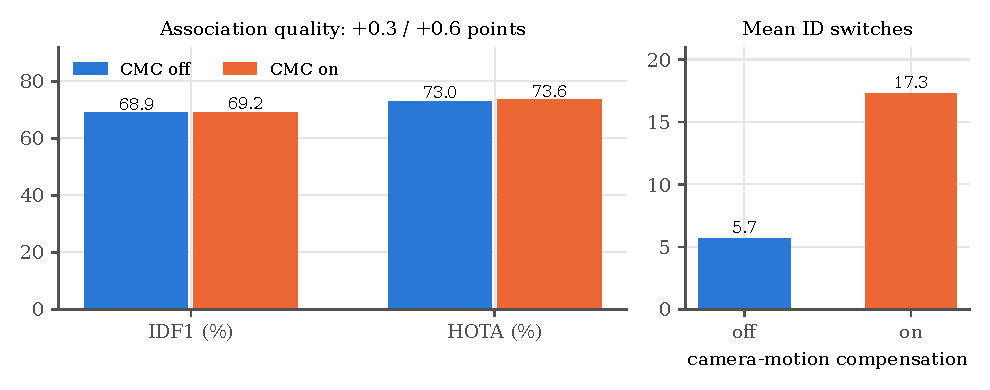
\includegraphics[width=.92\textwidth]{fig07_cmc_ablation.pdf}
\caption{Camera-motion compensation ablation (aggregate means over V1--V3, from Table~\ref{tab:cmc}). Left: IDF1 and HOTA. Right: mean identity switches (lower is better). Bars start at zero.}\label{fig:cmc}
\end{figure}
\noindent Figure~\ref{fig:cmc} shows two nearly equal pairs of association-quality bars next to a threefold increase in mean identity switches. The identity-quality metrics are essentially unchanged and the switch count is higher. We draw no causal conclusion about why: the source's per-video statement on this point is self-contradictory and per-video values are not reported (\todo{per-video CMC on/off values needed}). The source reports a median global shift of 0.3~px on V1 and 4.5~px on V2, yet labels all three videos ``static'', which is a further inconsistency.

\subsection{M3: counting accuracy}\label{sec:res-count}
Table~\ref{tab:count} compares the ByteTrack track count with the reference identity count.

\begin{table}[t]
\caption{Count accuracy for ByteTrack against the provisional ground truth (retained identities, Table~\ref{tab:gt}); Eq.~(\ref{eq:counterr}).}\label{tab:count}
\centering\small
\begin{tabular}{lrrrr}
\toprule
Video & GT identities & Predicted tracks & Absolute error & Error (\%)\\
\midrule
V1 & 9 & 10 & 1 & 11.1\\
V2 & 7 & 18 & 11 & 157.1\\
V3 & 14 & 17 & 3 & 21.4\\
\midrule
Mean / pooled & 10.0 / 30 & 15.0 / 45 & 5.0 / 15 & 63.2 / 50.0\\
\bottomrule
\end{tabular}
\end{table}

\begin{figure}[t]
\centering
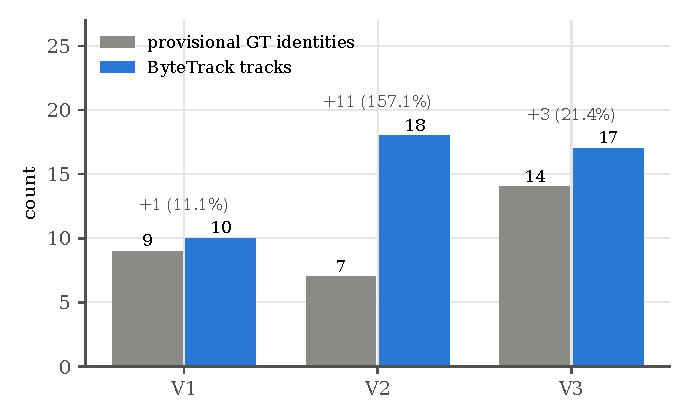
\includegraphics[width=.65\textwidth]{fig08_counting.pdf}
\caption{Reference identities and ByteTrack tracks per video; annotations give the signed error and relative error of Table~\ref{tab:count}.}\label{fig:count}
\end{figure}
\noindent Figure~\ref{fig:count} shows over-counting on every video, by 1, 11 and 3 tracks, and a pooled excess of 15 tracks on 30 reference identities. V2 is the hard case: ByteTrack produced more than twice as many tracks as there are reference identities. The source reports that the median track lasts 377 frames on V1 but 37 frames on V2, a clip of only 141 frames, and that V2 has a larger global camera shift (median 4.5~px against 0.3~px on V1; 95th percentile 44.7~px). These figures are consistent with fragmented tracks on V2, but our evidence does not separate camera motion from other causes. Two caveats apply to all rows: the reference is machine-generated (Section~\ref{sec:gt}), and the source does not state whether the predicted count applies a minimum-length filter comparable to the one that built the reference. If it does not, part of the excess may reflect the filter rather than tracker fragmentation.

\subsection{M1 and M3: sensitivity to the detection threshold}\label{sec:res-thr}
The detection-confidence threshold is the one threshold the offline harness can sweep end to end. Each video was re-run with ByteTrack at three thresholds between 0.25 and 0.75 (Figure~\ref{fig:thr}). The source reports that identity metrics are not measurably affected, while the predicted track count falls sharply as low-confidence detections are removed; it attributes the insensitivity of the metrics to ByteTrack's own high-confidence threshold. We report this as an observation from the source and have not independently verified the mechanism. A numeric table of this sweep is not available. \todo{Per-threshold table needed.}

\begin{figure}[t]
\centering
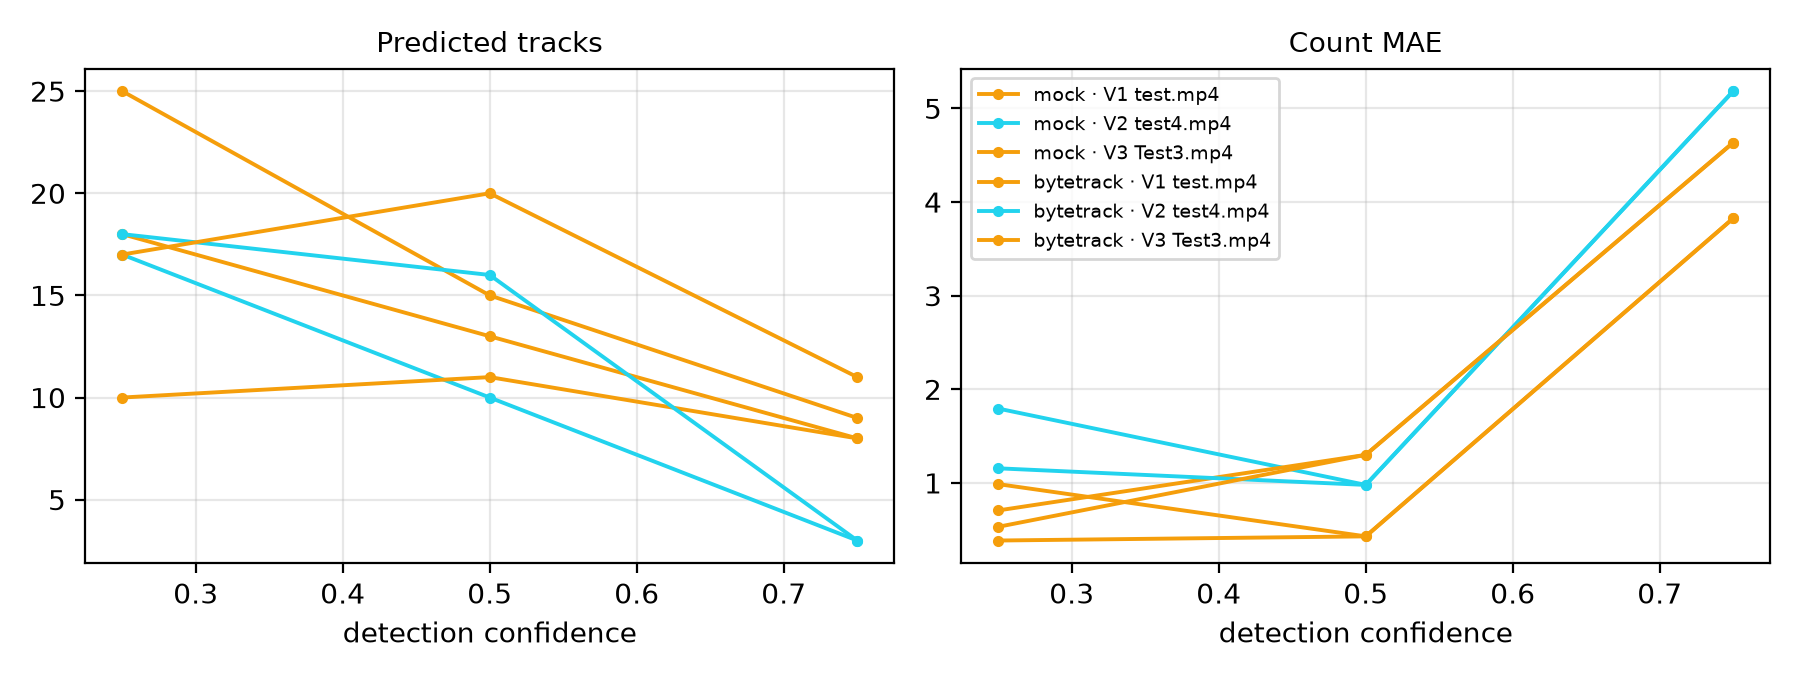
\includegraphics[width=\textwidth]{fig09_threshold_sweep.png}
\caption{Predicted track count (left) and count MAE (right) against the detection-confidence threshold on V1--V3 (original harness output; its legend uses the same colour for several curves).}\label{fig:thr}
\end{figure}
\noindent In Figure~\ref{fig:thr} the predicted track counts decrease as the threshold rises, from between about 10 and 25 tracks at 0.25 to between about 3 and 11 at 0.75. The count MAE curves are lowest at the low and middle thresholds and rise sharply between 0.5 and 0.75 for the curves visible there. Because the reference counts are 7--14, a track count near 3 at the highest threshold can only be an under-count, so a high threshold buys fewer duplicates at the price of missed fruit. The legend of the original plot does not distinguish all curves, so we do not attribute individual curves to trackers.

\subsection{Runtime}\label{sec:res-time}
Table~\ref{tab:runtime} summarises per-frame processing time over V1--V3. The time covers detection and tracking and excludes frame decoding; embedding extraction and identity matching are not included.

\begin{table}[t]
\caption{Processing time per frame, averaged over V1--V3, on the machine of Section~\ref{sec:setup}.}\label{tab:runtime}
\centering\small
\begin{tabular}{lrrr}
\toprule
Tracker & Mean (ms/frame) & 95th pct (ms) & Throughput (FPS)\\
\midrule
centre-distance & 25.8 & 28.8 & 39.0\\
ByteTrack & 25.3 & 28.6 & 39.5\\
TAPNext$^{\ddagger}$ & 600.0 & 700.0 & 1.67\\
\bottomrule
\end{tabular}\\[2pt]
{\footnotesize $^{\ddagger}$Unverified; the round values (600.0, 700.0) should be confirmed as measurements. The TAPNext row is not interpreted.}
\end{table}

\begin{figure}[t]
\centering
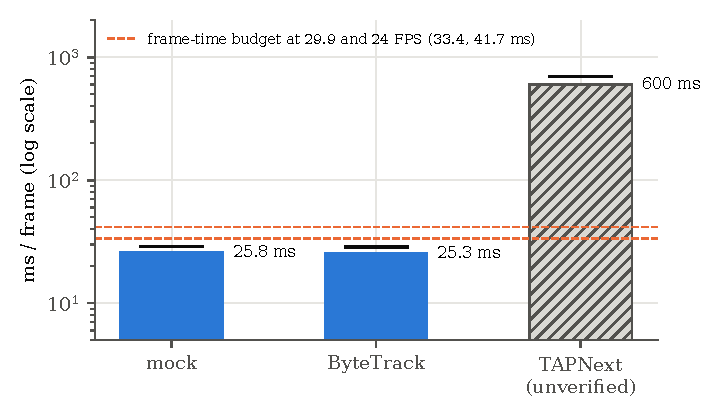
\includegraphics[width=.65\textwidth]{fig10_runtime.pdf}
\caption{Mean per-frame time (bars; horizontal ticks mark the 95th percentile) from Table~\ref{tab:runtime}, log scale. Dashed lines mark the frame-time budgets of the 24 and 29.9~FPS evaluation videos. The TAPNext bar is hatched because the values are unverified.}\label{fig:runtime}
\end{figure}
\noindent Figure~\ref{fig:runtime} shows that the centre-distance and ByteTrack back-ends sit below the frame-time budgets of the evaluation videos, at about 39 frames per second on this machine, while the unverified TAPNext figures are more than an order of magnitude above them. The cost of the embedder and identity memory is not measured.

\begin{figure}[t]
\centering
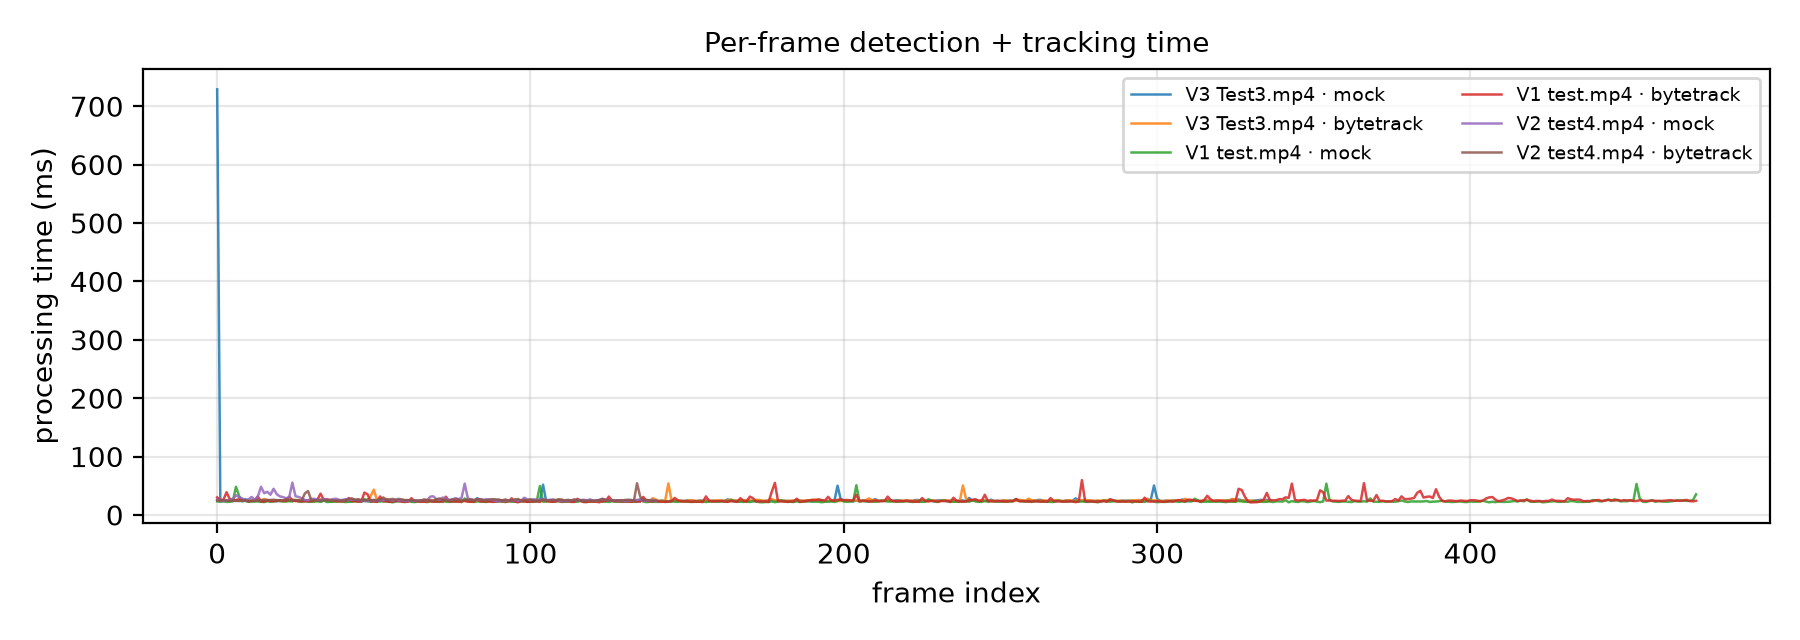
\includegraphics[width=.85\textwidth]{fig11_frame_time_trace.png}
\caption{Per-frame detection and tracking time over the three evaluation videos (original harness output).}\label{fig:trace}
\end{figure}
\noindent Figure~\ref{fig:trace} shows an isolated start-up spike above 700~ms on the first frame, after which the time per frame is roughly steady near the tabulated mean with occasional short peaks.

\subsection{Discussion}
We restrict interpretation to results that the provisional ground truth and the tabulated numbers can support.
\begin{description}[leftmargin=1.2em,style=nextline]
\item[Pipeline feasibility.] Detection plus ByteTrack runs faster than the frame rate of the evaluation videos on a laptop-class machine, so the pipeline is not computationally prohibitive at the detection-and-tracking level. This says nothing about the cost of the embedder or identity memory.
\item[Baseline versus ByteTrack.] The baseline scored a few points higher with fewer switches, from three videos, without variance estimates and against a detector-built reference. The data do not show a benefit of ByteTrack over simple association.
\item[Counting.] All three counts were above the reference, markedly so on V2. Over-counting is the direction expected from identity fragmentation, but since the reference removes short tracks and may itself under-count, the data cannot apportion the error between tracker fragmentation, reference construction and camera motion.
\item[Camera-motion compensation.] No clear benefit: IDF1 and HOTA moved by 0.3 and 0.6 points while identity switches rose from 5.7 to 17.3.
\item[Detection threshold.] The reported insensitivity of identity metrics, with a sharp change in track count, suggests the threshold mainly affects how many tracks are created; whether this holds for both trackers is unresolved.
\item[What cannot be concluded.] Because the identity memory is outside the evaluated loop, the results say nothing about whether re-identification reduces double-counting. Because the ReID sweep and TAPNext results are unverified, they support no conclusion. Three short videos from one recording condition do not support claims about generalisation.
\end{description}

% =====================================================================
\section{Statistical Analysis}\label{sec:stats}

Only quantities that follow from numbers printed in the source are analysed. The sample is $n=3$ videos, so the analysis is mainly descriptive, and its main purpose is to show how little the data can establish. All values below were computed from the per-video values of Section~\ref{sec:res-trk} and Table~\ref{tab:count}.

\paragraph{Descriptive statistics and intervals.} Table~\ref{tab:desc} gives mean, sample standard deviation and range for ByteTrack, and a $t$-based 95\% interval with $n-1=2$ degrees of freedom.

\begin{table}[t]
\caption{Descriptive statistics of ByteTrack over the three videos (sample SD, $n=3$) and 95\% $t$-intervals for the mean ($t_{0.975,2}=4.303$).}\label{tab:desc}
\centering\small
\begin{tabular}{lrrrrr}
\toprule
Metric & Mean & SD & Min--max & 95\% interval for mean & Possible range\\
\midrule
IDF1 (\%) & 69.0 & 40.5 & 22.6--97.0 & $-31.6$ to 169.6 & 0--100\\
HOTA (\%) & 73.0 & 34.7 & 33.3--96.9 & $-13.1$ to 159.2 & 0--100\\
ID switches & 5.7 & 3.5 & 2--9 & $-3.1$ to 14.4 & $\ge0$\\
\bottomrule
\end{tabular}
\end{table}

The intervals extend past the possible range of every metric, i.e.\ they are uninformative: with $n=3$ and a spread from 22.6 to 97.0, the mean IDF1 cannot be located. They also assume approximate normality, which cannot be checked with three points.

\paragraph{Paired comparison of identity switches.} For the only metric with exact per-video values for both trackers, the paired differences (ByteTrack minus baseline) are $+1$, $+6$ and $+7$. The mean difference is $+4.67$ switches (SD 3.21; 95\% interval $-3.3$ to $+12.7$); a paired $t$-test gives $t_2=2.51$, $p=0.128$. An exact Wilcoxon signed-rank test cannot give a two-sided $p$ below $0.25$ for $n=3$, even when all three differences have the same sign (as here: $p=0.25$). Neither test can reach conventional significance, so the consistent direction of the three differences is suggestive only.

\paragraph{Counting error.} All three videos over-count. An exact two-sided sign test gives $p=2\times(1/2)^3=0.25$ for 3 of 3 videos in one direction, which again cannot reach $0.05$ for $n=3$. Pooling gives 45 predicted tracks for 30 reference identities ($+50\%$); the mean relative error is 63.2\%, dominated by V2 (157.1\%). Absolute errors are 1, 11 and 3 (mean 5.0).

\paragraph{What was not computed.} No significance claim is made for IDF1 or HOTA differences between trackers, because per-video values exist only for ByteTrack. Correlation of tracking quality with camera shift is not computed, because the shift is reported for two of the three videos only. A bootstrap over three videos would be uninformative, and no data were simulated to fill the gap.

\paragraph{Reading Figure~\ref{fig:stats}.} Figure~\ref{fig:stats} is the visual counterpart of this section: the dots show the full distribution rather than a mean with error bars, which is the honest display at $n=3$.

% =====================================================================
\section{Ablation Study}\label{sec:ablation}

Table~\ref{tab:ablation} lists every component or configuration that the method description makes switchable, the experiment that would isolate it, and its status. Only the CMC ablation (Figure~\ref{fig:cmc}, Table~\ref{tab:cmc}) was run with an aggregate result, and the tracker choice and detection threshold were varied as reported in Section~\ref{sec:results}. Nothing in the other rows has been measured, and no values are shown for them.

\begin{table}[t]
\caption{Ablation configurations: what exists and what must be run. ``Not run'' rows contain no results by design.}\label{tab:ablation}
\centering\footnotesize
\begin{tabular}{p{3.0cm}p{4.0cm}p{3.1cm}p{3.6cm}}
\toprule
Component & Configurations to compare & Metrics & Status\\
\midrule
Camera-motion compensation (M5) & off vs.\ on & IDF1, HOTA, IDSW & Run, aggregate only (Table~\ref{tab:cmc}); per-video values missing\\
Tracker back-end (M2--M4) & centre-distance vs.\ ByteTrack vs.\ TAPNext & IDF1, HOTA, IDSW, count error & Run; TAPNext unverified\\
Detection threshold (M1) & three values in 0.25--0.75 & track count, count MAE, identity metrics & Run (ByteTrack), figure only; no table\\
Identity memory (M6) & tracker only vs.\ tracker + memory & count error, IDSW, IDF1 & Not run (memory outside the loop)\\
$\tau_{\mathrm{reid}}$ (M6) & several values & identities found, count error, false-link rate & Not run; source table unverified (App.~\ref{app:unresolved})\\
Motion gate / no-overlap rule (M6) & on vs.\ off & false links, count error & Not run\\
Observation-quality gate (M6) & threshold 0.3 vs.\ none & prototype stability, ReID accuracy & Not run\\
Embedder (M7) & stock ResNet-18 vs.\ fine-tuned & ReID accuracy, count error & Not run; no trained embedder evaluated\\
Reference construction & minimum-length filter on the prediction as on the reference & count error & Not run; filter symmetry unknown\\
\bottomrule
\end{tabular}
\end{table}

Of the rows with data, the only component-level result is negative for CMC: 0.3 and 0.6 points of IDF1 and HOTA against 11.6 additional identity switches (Figure~\ref{fig:cmc}). The remaining rows define the work required before any component can be said to contribute.

% =====================================================================
\section{Hypothesis Evaluation}\label{sec:hyp}

Figure~\ref{fig:hyp} states the mechanism that motivates the identity memory and the three hypotheses that the study can address.

\begin{figure}[t]
\centering
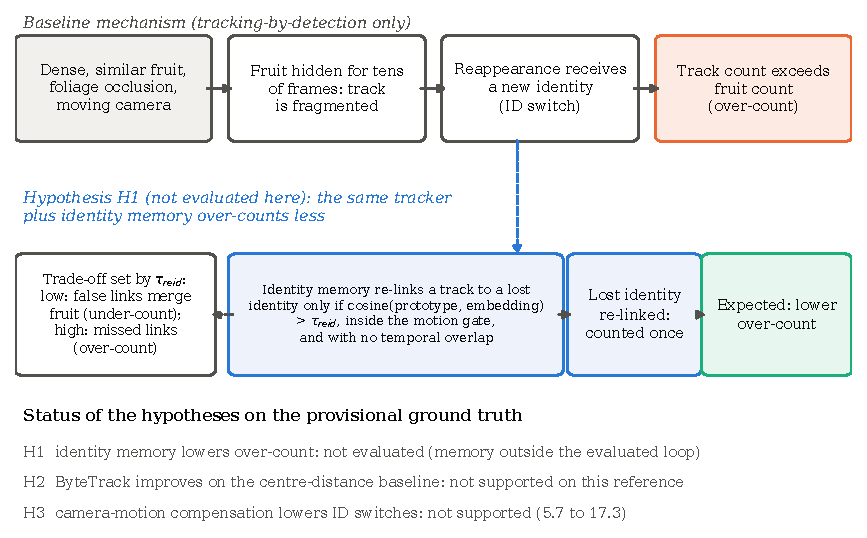
\includegraphics[width=\textwidth]{fig02_hypothesis.pdf}
\caption{Research hypothesis. Top: baseline mechanism by which occlusion causes fragmentation and over-counting. Middle: hypothesised effect of the identity memory (H1, not evaluated) and the trade-off controlled by $\tau_{\mathrm{reid}}$. Bottom: status of H1--H3 on the provisional reference.}\label{fig:hyp}
\end{figure}
\noindent Figure~\ref{fig:hyp} reads from the observed failure (over-counting by fragmentation, Section~\ref{sec:res-count}) to the mechanism proposed against it (re-linking by appearance and motion) and the error it can introduce (false links that merge two fruit). It is a statement of expectation, not of result. Table~\ref{tab:hyp} records how each hypothesis fared.

\begin{table}[t]
\caption{Hypotheses and their status on this evidence.}\label{tab:hyp}
\centering\footnotesize
\begin{tabular}{p{0.5cm}p{4.8cm}p{2.2cm}p{5.2cm}}
\toprule
ID & Hypothesis & Status & Evidence\\
\midrule
H1 & Identity memory added to a tracker lowers over-count & Not evaluated & Memory is outside the evaluated loop (Sec.~\ref{sec:setup}); needs the experiments of Table~\ref{tab:ablation}\\
H2 & ByteTrack improves association over centre-distance & Not supported on this reference & IDF1 69.0 vs.\ 70.9; HOTA 73.0 vs.\ 75.9; IDSW 5.7 vs.\ 1.0; $p=0.128$ (paired $t$), exact Wilcoxon $p=0.25$ for IDSW\\
H3 & CMC lowers identity switches & Not supported & IDSW 5.7 $\to$ 17.3; IDF1 and HOTA $+0.3$ / $+0.6$\\
H4 & The detection threshold changes the track count but not identity metrics & Observed in source, unverified & Summary statement and Figure~\ref{fig:thr}; no per-threshold table\\
\bottomrule
\end{tabular}
\end{table}

% =====================================================================
\section{Limitations}\label{sec:limits}
\begin{itemize}
\item \textbf{Provisional ground truth.} The reference is machine-generated from the same detector and not human-verified; identity metrics measure consistency with it, not absolute counting accuracy. Reference counts may under-count (Table~\ref{tab:gt}).
\item \textbf{Identity memory not evaluated.} The offline harness scores detection and tracking only. The system's central mechanism, prototype-based re-identification, has no validated result here.
\item \textbf{Embedder.} The embedder used is not trained on fruit; no trained embedder was evaluated.
\item \textbf{Unresolved results.} The ReID-threshold values and the TAPNext metrics (scale and units) are unverified and are not interpreted.
\item \textbf{Small, internally inconsistent dataset.} Three short videos, no variance beyond $n=3$; Table~\ref{tab:videos} was flagged incomplete in the source, and the ``static'' camera label conflicts with the reported camera motion. Count error appears under two definitions (Appendix~\ref{app:discrepancies}).
\item \textbf{Scope of identity matching.} Only short-term re-identification within a video is implemented; matching fruit across sessions or days is neither implemented nor evaluated.
\item \textbf{Deployment.} The system uses SQLite and local-disk storage and has not been evaluated under concurrent multi-user load.
\end{itemize}

% =====================================================================
\section{Global Impact and Future Directions}\label{sec:future}

\paragraph{Impact.} If identity errors can be isolated and reduced, video counting could complement manual sampling where tropical-fruit production is concentrated~\cite{fao_tropical}. Persisting every intermediate result matters here: for a grower or an agronomist, an unexplained count is less useful than one whose over- or under-count can be traced to fragmentation, a detector miss or a camera movement. The claim is limited to this diagnostic value; accuracy gains remain to be demonstrated.

\paragraph{Future work, in order of priority.}
\begin{enumerate}[label=(\roman*)]
\item Human verification of the ground truth and a larger, annotated, multi-season dataset.
\item Running the identity memory inside the evaluated loop, including the ReID-threshold sweep and a clear statement of which embedder is used.
\item Fine-tuning the embedder on fruit crops with a metric-learning loss~\cite{hermans2017triplet,oord2018cpc}.
\item Clarifying and re-running the TAPNext evaluation.
\item Linking identities across recording sessions to follow fruit through a season, which is not implemented here.
\item Depth or multi-camera information to resolve mutually occluding fruit.
\end{enumerate}

% =====================================================================
\section{Conclusion}\label{sec:conclusion}
We presented OrchardVision, an implemented pipeline for fruit tracking in orchard video that combines detection, interchangeable trackers, optional camera-motion compensation and a prototype-based identity memory, with all intermediate results persisted and a harness for tracker comparison. On three videos and a provisional, machine-generated reference, ByteTrack over-counted on all videos (pooled $+50\%$), a simple centre-distance baseline performed comparably to it, and camera-motion compensation gave no clear benefit while tripling identity switches. With $n=3$ videos none of these differences can be established statistically (smallest attainable exact $p$ is 0.25). These findings concern tracker consistency; absolute counting accuracy, the benefit of the identity memory, and the TAPNext and ReID-threshold results remain unvalidated.

% =====================================================================
\appendix
\section{Unresolved Material (Not Evidence)}\label{app:unresolved}

The source report contains a populated ReID-threshold table whose caption describes different columns from its headings, and whose provenance is unconfirmed. It also states that such a sweep requires the identity memory to be in the evaluated loop, which the offline harness does not currently do. Table~\ref{tab:reid} reproduces the printed values for transparency only; \textbf{they are not evidence and nothing in this paper depends on them.}

\begin{table}[t]
\caption{Unresolved; provenance unconfirmed. ReID-threshold values as printed in the source report (averaged over V1--V3). Do not cite as a result.}\label{tab:reid}
\centering\small
\begin{tabular}{rrrr}
\toprule
ReID threshold & Identities found & IDF1 & ID switches\\
\midrule
0.90 & 13.3 & 3.7 & 11\\
0.93 & 14.3 & 2.7 & 12\\
0.95 & 15.7 & 1.3 & 13\\
0.97 & 17.0 & 0.0 & 17\\
\bottomrule
\end{tabular}
\end{table}

\begin{figure}[t]
\centering
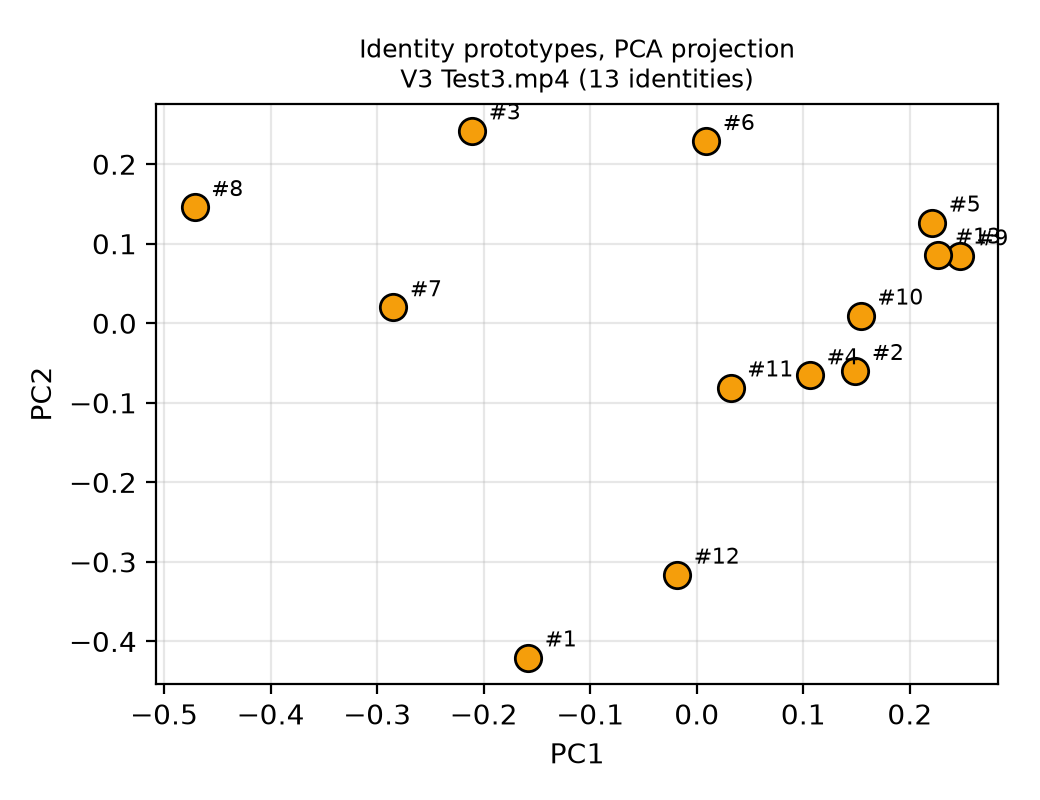
\includegraphics[width=.6\textwidth]{fig12_identity_pca.png}
\caption{Two-dimensional PCA projection of identity prototypes (unresolved; not interpreted). The plot title reads ``V3 Test3.mp4 (13 identities)'', whereas the earlier caption attributed it to V2.}\label{fig:pca}
\end{figure}
\noindent Figure~\ref{fig:pca} is shown only for completeness. We make no claim about how well identity prototypes separate, because that depends on which embedder was used and on whether the plotted run is the one stated. The source's illustrative re-identification example refers to a video labelled V4, which is not in the evaluation set (Table~\ref{tab:videos}), and is omitted.

\section{Source Discrepancies and How They Were Handled}\label{app:discrepancies}

\begin{table}[t]
\caption{Discrepancies in the source material and their treatment.}\label{tab:disc}
\centering\footnotesize
\begin{tabular}{p{4.2cm}p{5.2cm}p{4.5cm}}
\toprule
Item & Observation & Treatment\\
\midrule
Count error, Table~\ref{tab:trackers} (0.61) vs.\ Table~\ref{tab:count} (absolute errors 1, 11, 3; mean 5.0) & Different magnitudes and units. Mean relative error from Table~\ref{tab:count} is 0.63 (63.2\%), not 0.61, so the tables may stem from different runs. The magnitude of 0.61 resembles the count-MAE curves of Figure~\ref{fig:thr} (about 0.3--1.8 at low thresholds), which suggests, but does not establish, a per-frame count error & Table~\ref{tab:trackers} retains the column with its caveat; counting analysis uses Table~\ref{tab:count}\\
ByteTrack IDF1 69.0 (Table~\ref{tab:trackers}) vs.\ 68.9 (Table~\ref{tab:cmc}) & Per-video mean is 68.987; 68.9 is a truncation & Both kept; footnote in Table~\ref{tab:cmc}\\
Original Figure~5 & Plot labelled ``static'' with per-video ByteTrack bars; it did not compare CMC on and off. Its labelled values reproduce the CMC-off means & Per-video values used in Figure~\ref{fig:stats}; new Figure~\ref{fig:cmc} drawn from Table~\ref{tab:cmc}\\
Original Figure~8 caption (V2) vs.\ plot title (V3, 13 identities) & Conflict & Reported in Figure~\ref{fig:pca}\\
Original Figure~1 & Showed operator steps, not data flow, under a pipeline caption & Replaced by Figure~\ref{fig:pipeline}\\
Throughput, centre-distance row & $1000/25.8=38.8$ FPS against 39.0 printed & Printed values kept\\
Embedder training & Contradictory statements in source & Only the untrained extractor is reported (Section~M7)\\
Reference to InfoNCE & Earlier report cited a ``loss function for deep metric learning'' (Reddi et~al., ICCV 2017), which we could not find; InfoNCE originates in~\cite{oord2018cpc} & Citation replaced\\
CMC per-video statement (``9 to 36'' on V1) & Contradicts V1 switch count of 2 in the source figures; the value 9 coincides with the V3 CMC-off count & Not used\\
\bottomrule
\end{tabular}
\end{table}

% =====================================================================
\begin{thebibliography}{99}\small
\bibitem{aharon2022botsort} N.~Aharon, R.~Orfaig, and B.-Z. Bobrovsky. BoT-SORT: Robust associations multi-pedestrian tracking. \emph{arXiv preprint arXiv:2206.14651}, 2022.
\bibitem{bargoti2017deep} S.~Bargoti and J.~Underwood. Deep fruit detection in orchards. In \emph{Proc.\ IEEE Int.\ Conf.\ Robotics and Automation (ICRA)}, pages 3626--3633. IEEE, 2017.
\bibitem{bayer2012sqlalchemy} M.~Bayer. SQLAlchemy. In A.~Brown and G.~Wilson, editors, \emph{The Architecture of Open Source Applications, Volume II}. aosabook.org, 2012.
\bibitem{bernardin2008clear} K.~Bernardin and R.~Stiefelhagen. Evaluating multiple object tracking performance: The CLEAR MOT metrics. \emph{EURASIP Journal on Image and Video Processing}, 2008:Article 246309, 2008.
\bibitem{bewley2016sort} A.~Bewley, Z.~Ge, L.~Ott, F.~Ramos, and B.~Upcroft. Simple online and realtime tracking. In \emph{Proc.\ IEEE Int.\ Conf.\ Image Processing (ICIP)}, pages 3464--3468. IEEE, 2016.
\bibitem{doersch2022tapvid} C.~Doersch, A.~Gupta, L.~Markeeva, A.~Recasens, L.~Smaira, Y.~Aytar, J.~Carreira, A.~Zisserman, and Y.~Yang. TAP-Vid: A benchmark for tracking any point in a video. In \emph{Advances in Neural Information Processing Systems (NeurIPS), Datasets and Benchmarks Track}, 2022.
\bibitem{ester1996dbscan} M.~Ester, H.-P. Kriegel, J.~Sander, and X.~Xu. A density-based algorithm for discovering clusters in large spatial databases with noise. In \emph{Proc.\ Second Int.\ Conf.\ Knowledge Discovery and Data Mining (KDD)}, pages 226--231. ACM, 1996.
\bibitem{fao_tropical} Food and Agriculture Organization of the United Nations. Commodity in focus: Tropical fruits. \url{https://www.fao.org/markets-and-trade/commodities/tropical-fruits}. Accessed 22 November 2026.
\bibitem{hermans2017triplet} A.~Hermans, L.~Beyer, and B.~Leibe. In defense of the triplet loss for person re-identification. \emph{arXiv preprint arXiv:1703.07737}, 2017.
\bibitem{jolliffe2016pca} I.~T. Jolliffe and J.~Cadima. Principal component analysis: A review and recent developments. \emph{Philosophical Transactions of the Royal Society A}, 374(2065):20150202, 2016.
\bibitem{kalman1960} R.~E. Kalman. A new approach to linear filtering and prediction problems. \emph{Journal of Basic Engineering}, 82(1):35--45, 1960.
\bibitem{koirala2019review} A.~Koirala, K.~B. Walsh, Z.~Wang, and C.~McCarthy. Deep learning -- method overview and review of use for fruit detection and yield estimation. \emph{Computers and Electronics in Agriculture}, 162:219--234, 2019.
\bibitem{kuhn1955} H.~W. Kuhn. The Hungarian method for the assignment problem. \emph{Naval Research Logistics Quarterly}, 2(1--2):83--97, 1955.
\bibitem{liu2019monocular} X.~Liu, S.~W. Chen, C.~Liu, S.~S. Shivakumar, J.~Das, C.~J. Taylor, J.~Underwood, and V.~Kumar. Monocular camera based fruit counting and mapping with semantic data association. \emph{IEEE Robotics and Automation Letters}, 4(3):2296--2303, 2019.
\bibitem{luiten2021hota} J.~Luiten, A.~Osep, P.~Dendorfer, P.~Torr, A.~Geiger, L.~Leal-Taix\'e, and B.~Leibe. HOTA: A higher order metric for evaluating multi-object tracking. \emph{International Journal of Computer Vision}, 129(2):548--578, 2021.
\bibitem{oord2018cpc} A.~van~den Oord, Y.~Li, and O.~Vinyals. Representation learning with contrastive predictive coding. \emph{arXiv preprint arXiv:1807.03748}, 2018.
\bibitem{fastapi} S.~Ram\'irez. FastAPI [computer software]. \url{https://fastapi.tiangolo.com}. No date given in the source report.
\bibitem{redmon2016yolo} J.~Redmon, S.~Divvala, R.~Girshick, and A.~Farhadi. You only look once: Unified, real-time object detection. In \emph{Proc.\ IEEE Conf.\ Computer Vision and Pattern Recognition (CVPR)}, pages 779--788. IEEE, 2016.
\bibitem{ristani2016idf1} E.~Ristani, F.~Solera, R.~Zou, R.~Cucchiara, and C.~Tomasi. Performance measures and a data set for multi-target, multi-camera tracking. In \emph{European Conference on Computer Vision Workshops}, pages 17--35. Springer, 2016.
\bibitem{vandermaaten2008tsne} L.~van~der Maaten and G.~Hinton. Visualizing data using t-SNE. \emph{Journal of Machine Learning Research}, 9(Nov):2579--2605, 2008.
\bibitem{wang2019mango} Z.~Wang, K.~Walsh, and A.~Koirala. Mango fruit load estimation using a video based MangoYOLO--Kalman filter--Hungarian algorithm method. \emph{Sensors}, 19(12):2742, 2019.
\bibitem{wojke2017deepsort} N.~Wojke, A.~Bewley, and D.~Paulus. Simple online and realtime tracking with a deep association metric. In \emph{Proc.\ IEEE Int.\ Conf.\ Image Processing (ICIP)}, pages 3645--3649. IEEE, 2017.
\bibitem{ultralytics} YOLO Team and Ultralytics. Ultralytics YOLO [computer software]. \url{https://github.com/ultralytics/ultralytics}, 2024.
\bibitem{zhang2022bytetrack} Y.~Zhang, P.~Sun, Y.~Jiang, D.~Yu, F.~Weng, Z.~Yuan, P.~Luo, W.~Liu, and X.~Wang. ByteTrack: Multi-object tracking by associating every detection box. In \emph{European Conference on Computer Vision (ECCV)}, pages 1--21. Springer, 2022.
\bibitem{zholus2025tapnext} A.~Zholus, C.~Doersch, Y.~Yang, S.~Koppula, V.~Patraucean, X.~O. He, I.~Rocco, M.~S.~M. Sajjadi, S.~Chandar, and R.~Goroshin. TAPNext: Tracking any point (TAP) as next token prediction. \emph{arXiv preprint arXiv:2504.05579}, 2025.
\end{thebibliography}

\end{document}
